\chapter{Modelagem matemática}

\section{Modelagem matemática}

Dentro da pesquisa, foram realizadas duas modelagens distintas, ambas, diferentemente da literatura clássica, foram elaboradas com base nas estações de origem e destino, e não nos legs do percurso.

Para compreender essas propostas, consideremos uma versão simplificada do problema, onde temos:

\begin{enumerate}[label=\textbullet]
	\item 4 estações pelas quais o trem deve passar em um único sentido, ou seja, o trem não tem retorno.
	\item O trem tem uma capacidade máxima de assentos.
	\item Há apenas um tipo de classe comercial.
	\item Existe apenas um período no horizonte de reserva.
	\item A variável de decisão é a quantidade de assentos que pode ser disponibilizada para venda em um trecho com origem e destino específicos.
	\item Todos os assentos disponibilizados para venda serão vendidos.
\end{enumerate}

A figura \ref{fig: fig1} apresenta graficamente a situação proposta:

\begin{figure}[th]
	\begin{center}
		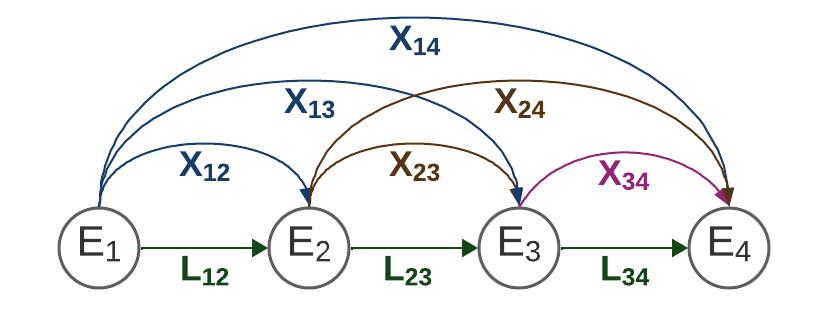
\includegraphics[]{img/fig1.png}
		\caption{Versão gráfica simples}
		% Fonte:~\cite{khaksar2013genetic}}
		\label{fig: fig1}
	\end{center}
\end{figure}



\section{Primeira modelagem matemática}\label{sec:modelo1}
Dentro da pesquisa, foram realizadas duas modelagens distintas, ambas, diferentemente da literatura clássica, foram elaboradas com base nas estações de origem e destino, e não nos legs do percurso.

Para compreender essas propostas, consideremos uma versão simplificada do problema, onde temos:

